\section{Язык Дика на одном типе скобок}\label{section:dyck_1}

Вспомним алгоритм~\ref{algo:PI}. Его слабым местом, дающим кубическую нижнюю оценку, было поддержание инкрементального транзитивного замыкания. Проблемы была в том, что рёбра могли добавляться по одному, и тогда никаким более простым/быстрым методом было не справиться. Однако, если новые пути появляются не по-одному, а сразу большими группами, задачу можно решать эффективнее.

\subsection{Алгоритм, основанный на неикрементальном транзитивном замыкании}\label{subsection:nitc}

Ключом к более быстрому решению является построение транзитивного замыкания с нуля на каждой итерации алгоритма. И, так как обычное транзитивное замыкание можно найти за субкубическое время, то если итераций алгоритма немного, такое решение получается асимптотически быстрее основного (алгоритма~\ref{algo:PI}).

В листинге~\ref{algo:P} приведён псевдокод решения.

\begin{algorithm}[h]
    \floatname{algorithm}{Listing}
    \begin{algorithmic}[1]
    \caption{Алгоритм достижимости для РКА}
    \label{algo:P}
    \Function{RSMReachability}{$\cool{R}$}
        \State{$A \gets$ Adjacency matrix for $\cool{R}$}
        \While{$A$ is changing}
            \State{$A' \gets \textit{transitiveClosure}(A)$}
            \Comment{Построение транзитивного замыкания}
            \For{$i \in 1..k$}
               \For{$u \in En_i$}
                    \For{$v \in Ex_i$}
                        \If{$A'_{u,v} \wedge \overline{A_{u,v}}$}
                            \State{$A' \gets A' \cup getEdges(i, u, v)$}
                            \Comment{Добавление новых рёбер}
                        \EndIf
                    \EndFor
               \EndFor
            \EndFor
            \State{$A \to A'$}
        \EndWhile
    \State \Return $A$
    \EndFunction
    \end{algorithmic}
\end{algorithm}

Изначально, так же, как и в алгоритме~\ref{algo:PI}, в матрицу смежности $A$ записываются все внутренние рёбра РКА $\cool{R}$.

Далее, внешний цикл повторяется, пока матрица смежности $A$ меняется (т.е. пока добавляются новые рёбра). На каждой итерации считается $A'$~--- транзитивное замыкание $A$. После этого находятся все новые пути вида $\langle$стартовое состояние$\rangle$ $\path$ $\langle$конечное состояние$\rangle$~--- те рёбра между стартовой и конечной вершинами компоненты, которых не было в $A$, но которые есть в $A'$~--- и добавляются соответствующие этим путям рёбра.

\subsubsection*{Время работы}

Время работы алгоритма~--- $k \cdot T(|V|)$, где $k$~--- число итераций внешнего цикла, $T(|V|)$~--- время работы одной итерации. 

Оценим $T(|V|)$. Внутренняя часть цикла состоит из двух частей: нахождения транзитивного замыкания (строка 4) и прохода по матрице для выявления новых рёбер (строки 5-9). 

Задача поиска транзитивного замыкания эквивалентна задаче перемножения булевых матриц~\cite{Aho1974} и может быть решена сведением к быстрому перемножению (обычных) матриц за $\O(|V|^\omega)$.

Проход по матрице (строки 5-7) работает за $\O(|V|^2)$, что доминируется временем построения транзитивного замыкания. Добавление новых рёбер (строки 8-9) отработает суммарно за $\O(|V|^2)$ (так как каждое ребро будет добавлено не более одного раза).

Итого, время работы алгоритма составляет $\O(k \cdot |V|^{\omega})$.

\subsection{Алгоритм для языка Дика на одном типе скобок}

\begin{definition}\label{def:dyck_paths}
  Строки, принадлежащие языку Дика $\cool{D}_1$ часто изображают в виде \textit{путей Дика}~--- путей из точки $(0, 0)$ в точку $(0, 2n)$, не опускающихся ниже оси абсцисс. Открывающей скобке соответствует вектор $(1, 1)$, закрывающей~--- $(1, -1)$.

  Части путей, образованные строками вида $(^k )^k$ будем называть \textit{горами}.

\end{definition}

\begin{figure}[h]
  \begin{tikzpicture}[scale=0.6]
    \draw[help lines, color=gray!30, dashed] (-0.5,-0.5) grid (24.5,5.5);
    \draw[->,ultra thick] (-0.5,0)--(24.5,0) node[right]{$x$};
    \draw[->,ultra thick] (0,-0.5)--(0,5.5)  node[above]{$y$};

    \edef\x{0}
    \edef\y{0}

    \newcommand\up{}
    \def\up{%
      \draw[->,thick] (\x,\y)--++(1,1); 
      \pgfmathparse{\x+1}
      \edef\x{\pgfmathresult}
      \pgfmathparse{\y+1}
      \edef\y{\pgfmathresult}
    }

    \newcommand\down{}
    \def\down{%
      \draw[->,thick] (\x,\y)--++(1,-1); 
      \pgfmathparse{\x+1}
      \edef\x{\pgfmathresult}
      \pgfmathparse{\y-1}
      \edef\y{\pgfmathresult}
    }

    \up; \up; \up; \up; \up;
    \down; \down; \down; \down;
    \up; \up; \up;
    \down; \down; \down; \down;
    \up; \up; \up;
    \down;
    \up;
    \down; \down; \down;

  \end{tikzpicture}
  \caption{Путь Дика для строки \texttt{((((())))((())))((()()))}}
  \label{img:dyck_path}
\end{figure}

Для построения алгоритма воспользуемся следующим результатом:

\begin{lemma}[Дюлеаж и Лоран~\cite{Deleage1986}]\label{lm:french}

  Для языка $L$ определим \textit{рациональный индекс языка} $L$~--- $p_L(n)$\footnote{Формально, $p_L(n) = \max \{ \min \{|w| \colon w \in L \cap K \}, K \in Rat_n(X), L \cap K \ne \varnothing \}$,\\ где $Rat_n(X)$~--- регулярные языки над алфавитом $X$, распознаваемые НКА с $\le n$ состояниями.} как максимальную длину кратчайшего слова в $L \cap K$ по всем регулярным языкам $K$, задаваемым НКА с $\le n$ состояниями.

  Тогда для языка Дика $\cool{D}_1$ на одном типе скобок $p_{\cool{D}_1}(n) = \O(n^2)$\footnote{Точная оценка~--- $2n^2 + 4n$}
\end{lemma}

\begin{corollary}
  Для любой пары вершин $u, v \in V(G)$, если есть Диков путь $u \path v$, то существует и Диков путь $u \path v$, длина которого $\O(|V|^2)$.
\end{corollary}
\begin{proof}
  Слова, читаемые на путях $u \path v$ задаются НКА на $n$ вершинах~--- графом $G$, в котором $u$ и $v$ выбраны за начальное и конечное состояния соответственно.
\end{proof}

\begin{note}
  Пользуясь этим фактом, можно построить наивный алгоритм~--- достаточно лишь заметить, что раз длина искомого пути всегда ограничена, то можно задать такие пути с помощью автомата: язык $\cool{D}_1$ задаётся автоматом с одним счётчиком, значение счётчика не превышает $\O(|V|^2)$, так что его можно закодировать в состояние. Однако и размер такого автомата будет $\O(|V|^2)$, что для данной задач слишком много.
\end{note} 

\begin{note}\label{fact:regular_cfpq}
  Вообще, для любого регулярного языка задача CFPQ решается построением обычного транзитивного замыкания от графа-произведения, то есть за $\O(|V|^{\omega} |\cool{A}|^{\omega})$, где $|\cool{A}|$~--- число состояний автомата.
\end{note}

Наивный алгоритм имеет такое большое время работы из-за большого размера автомата. Воспользовавшись же алгоритмом~\ref{algo:P} можно построить более быстрое решение. Тем более известно, что часто размеры грамматик и автоматов для одних и тех же языков отличаются в экспоненциальное число раз.

Заметим, что для этого придётся видоизменить грамматику, для её стандартного вида ($\cool{D}_1 \colon S \to SS | ( S ) | \eps$) алгоритм~\ref{algo:P} может совершить до $\O(|V|^2)$ итераций: например, на цепочке $(^k )^k$ за одну итерацию будет проводиться лишь одно новое ребро (используя продукцию $S \to ( S )$), так что потребуются все $k$ итераций.

Другое представление языка $\cool{D}_1$ основано на двух \sout{китах} замечаниях: длина максимального слова всего $\O(|V|^2)$, хочется ``сжимать'' длинные горы (\ref{def:dyck_paths}) быстрее, чем за их длину.

\subsubsection{Грамматика для языка $\cool{D}_1$}

Пусть $K = \lceil \log (2 n^2 + 4n) \rceil$ (т.е. это логарифм длины максимального слова), построенная грамматика будет иметь размер $\O(K)$.

Грамматика будет содержать $2K$ нетерминалов, отвечающих за сжатие вертикальных путей: $U_i$ сжимает пути вида $(^{2^i}$, $D_i$ сжимает пути вида $)^{2^i}$:

\begin{align*}\label{eq:U}
  U_0 &\to ( \\
  U_1 &\to U_0\, S\, U_0 \\
  U_2 &\to U_1\, S\, U_1 \\
  &\dots \\
  U_K &\to U_{K-1}\, S\, U_{K-1} 
\end{align*}

В продукции для $U_i$ есть $S$ между $U_{i-1}$ и $U_{i-1}$~--- она нужна, $U_i$ ищет не строго возрастающие пути, а разрешает им некоторое время ``идти прямо'' (получаются уже такие пути Моцкина~\cite{Donaghey1977}, а не Дика, в которых рёбра с метками $S$ соответствуют горизонтальным рёбрам).

Продукции для $D_i$ устроены аналогично.

Теперь можем строить нетерминал, отвечающую за, собственно, пути Дика. Продукция $S \to ( S )$ в обычной грамматике как бы сжимала вершину горы. Теперь, пользуясь $U_i$ и $D_i$ она может сжимать горы побольше.

\begin{equation}\label{eq:S}
  \cool{D}_1 \colon S \to U_0\, S\, D_0~|~U_1\, S\, D_1~|~ \dots ~|~U_K\, S\, D_K~|~SS~\eps
\end{equation}

Для того, чтобы число итераций алгоритма~\ref{algo:P} было небольшим, РКА по данной грамматике нужно строить не совсем стандартным образом.

Так, продукция $S \to SS$ отвечает за транзитивное замыкание рёбер с $S$-метками. В случае РКА этого можно добиться, проведя $S$-петлю на терминальной вершине РКА (обозначим это как продукцию $S \to S^*$.

Также, при оценке асимптотики алгоритма будет важно, что все компоненты РКА имеют константный размер, так что компонента $S$ будет разбита на $K$ штук: $S_i \to U_i S D_i$ для всех $0 \le i \le K$, а также $S \to (S_0~|~S_1~|~ \dots ~|~ S_k)^*$ (одно стартовое/терминальное состояние, на котором весит $K$ петель), теперь эта компонента целиком отвечает только за транзитивное замыкание $S$-меток.

\begin{figure}[H]
    \begin{minipage}[h]{0.47\linewidth}
        \center{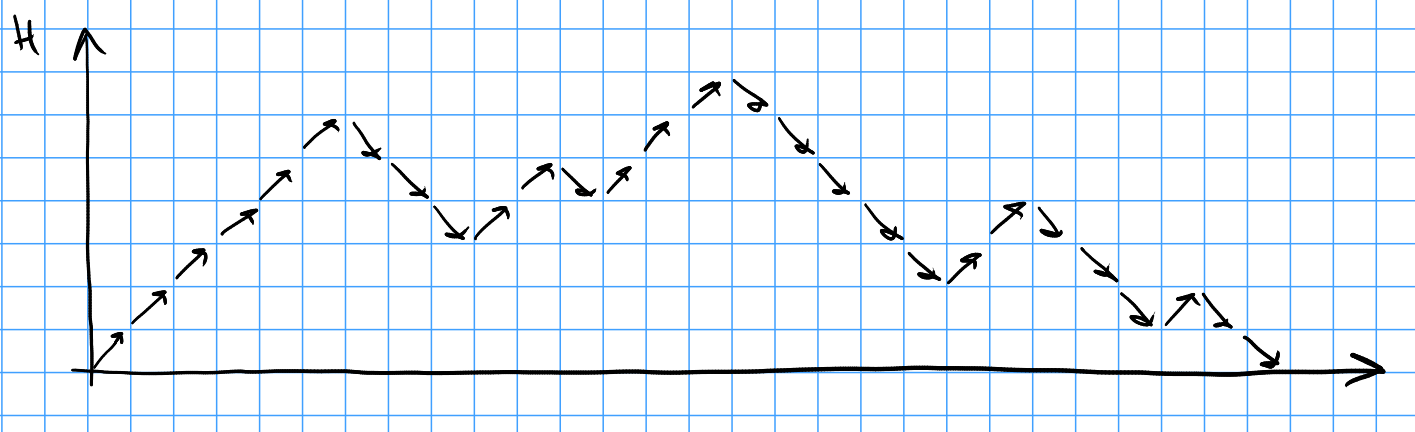
\includegraphics[width=1\linewidth]{img/dyck1_example/phase0}} 0 итерация
    \end{minipage}
    \hfill
    \begin{minipage}[h]{0.47\linewidth}
        \center{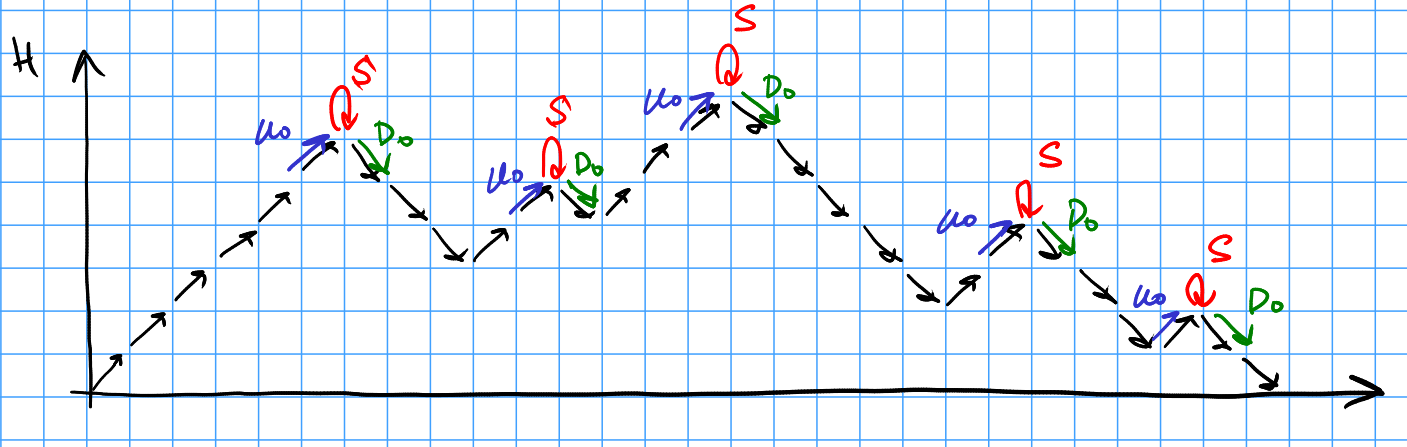
\includegraphics[width=1\linewidth]{img/dyck1_example/phase1}} 1 итерация
    \end{minipage}
    \vfill
    \begin{minipage}[h]{0.47\linewidth}
        \center{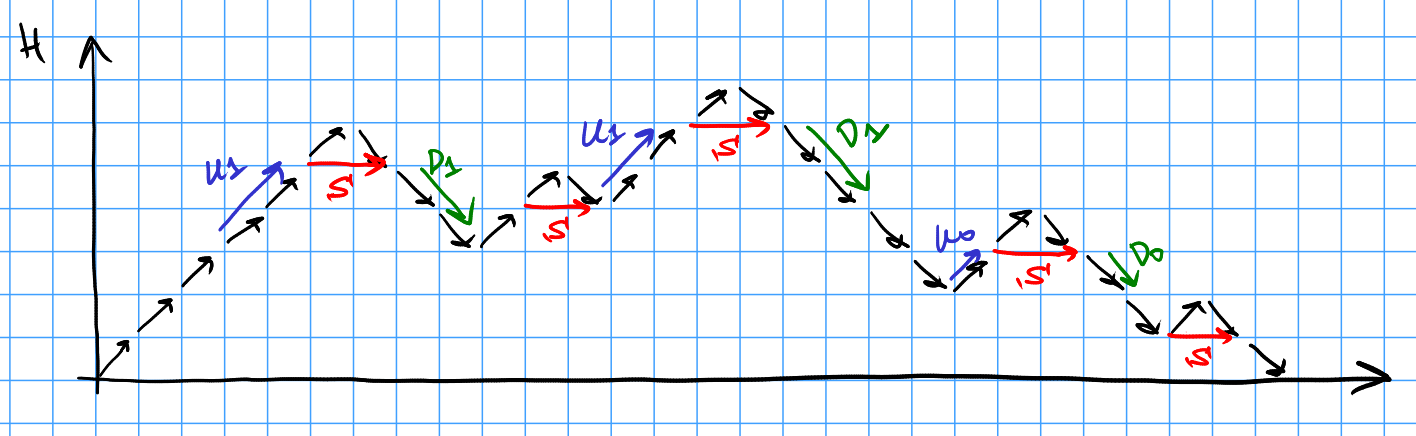
\includegraphics[width=1\linewidth]{img/dyck1_example/phase2}} 2 итерация
    \end{minipage}
    \hfill
    \begin{minipage}[h]{0.47\linewidth}
        \center{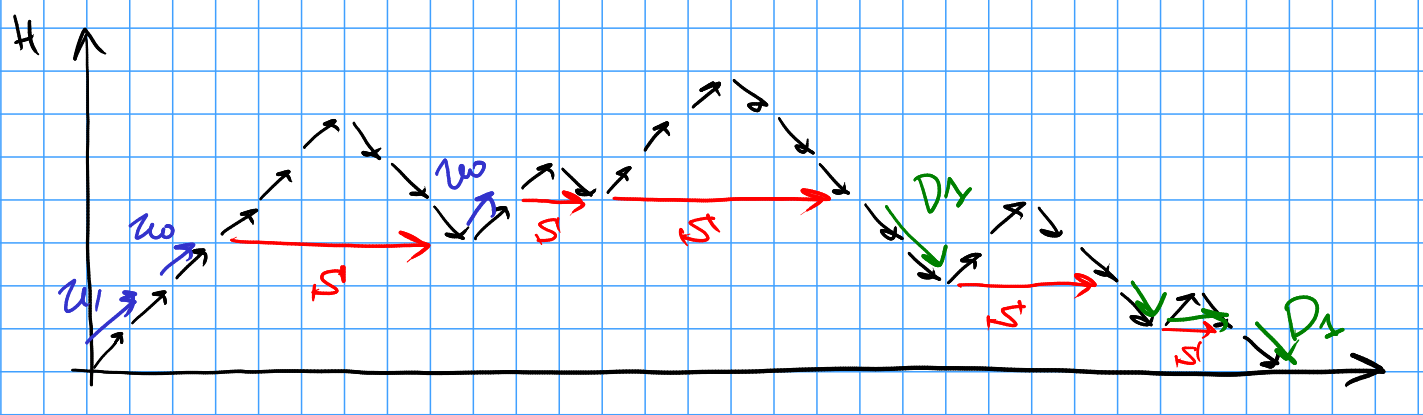
\includegraphics[width=1\linewidth]{img/dyck1_example/phase3}} 3 итерация
    \end{minipage}
    \vfill
    \begin{minipage}[h]{0.47\linewidth}
        \center{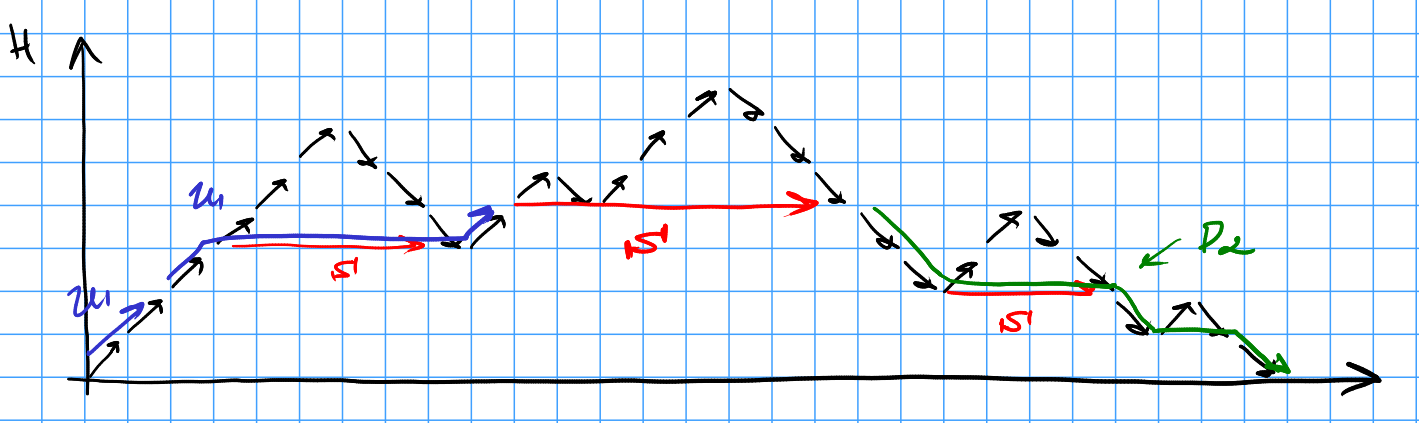
\includegraphics[width=1\linewidth]{img/dyck1_example/phase4}} 4 итерация
    \end{minipage}
    \hfill
    \begin{minipage}[h]{0.47\linewidth}
        \center{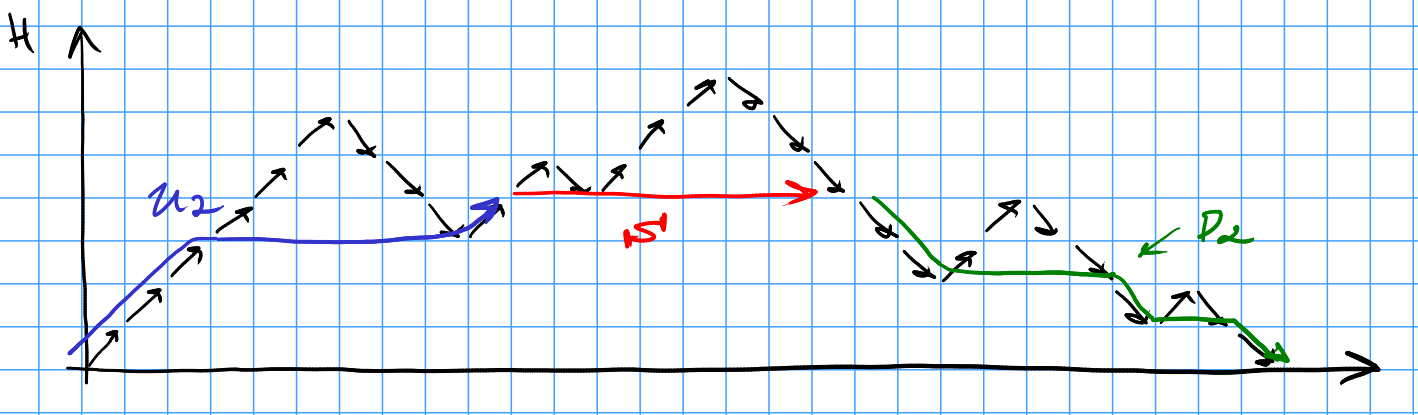
\includegraphics[width=1\linewidth]{img/dyck1_example/phase5}} 5 итерация
    \end{minipage}

    \caption{Пример работы алгоритма (на конкретном пути)}
    \label{img:dyck1_example}
\end{figure}

\TODO: норм картиночька

\subsubsection{Корректность алгоритма}

Посмотрим на нетерминал $S$ (опр.~\ref{eq:S}). В нём присутствуют все продукции из стандартного вида грамматики для языка $\cool{D}_1$, так что нужно доказать лишь, что все строки, которые выводятся остальными продукциями тоже являются корректными. 

Индукцией по длине строки несложно доказать, что:

\vspace{-\topsep}
\begin{enumerate}
  \setlength\itemsep{-0.1em}
  \item $U_i$ выводит корректные (с балансом на всех префиксах $\ge 0$) строки с балансом $2^{i}$
  \item $D_i$ выводит корректные (с балансом на всех префиксах $\ge -2^{i}$) строки с балансом $(-2^{i})$
  \item $S$ выводит корректные ПСП из $\cool{D}_1$
\end{enumerate}

База очевидна, переход тоже.

\subsubsection{Время работы}

\begin{theorem}
  Время работы алгоритма~\ref{algo:P} для языка Дика на одном типе скобок~--- $\O(|V|^{\omega} \log^3 |V|)$.
\end{theorem}

\begin{proof}
  Время работы алгоритма~\ref{algo:P} состоит из двух множителей: времени работы одной итерации и числа итераций.

  Время работы одной итерации в алгоритме~\ref{algo:P} составляло $\O(N^{\omega})$ (где $N$~--- число состояний РКА-произведения), так как на каждой итерации считалось транзитивное замыкание. Заметим, что на самом деле достаточно находить транзитивное замыкание отдельно в каждой компоненте РКА (так как разные компоненты вообще не связны). Поскольку компоненты РКА грамматики константны, размер компонент РКА-произведения~--- $\O(|V|)$. Так что суммарное время работы одной итерации составит $\O(|V|^{\omega} K)$.

  Оценим теперь число итераций. Рассмотрим конкретный путь (= строку) и посчитаем, сколько итераций потребуется, чтобы его сжать.

  Покажем, что все горы исходной строки сожмутся за $2K$ итераций. Длина горы $l$ раскладывается на сумму степеней двойки: $l = a_0 \cdot 1 + a_1 \cdot 2 + \dots + a_K \cdot 2^{K}$, где $a_i \in \{0, 1\}$. Покажем по индукции, что после $(2i+2)$-ого шага будет сжата в $S$-ребро верхушка горы длины $a_0 \cdot 1 + a_1 \cdot 2 + \dots + a_{i-1} \cdot 2^{i-1}$. База очевидна, переход: знаем, что на $2i$-ом шаге сжалась верхушка размера $a_0 \cdot 1 + a_1 \cdot 2 + \dots + a_{i-2} \cdot 2^{i-2}$, то есть остаётся только сжать в $S$-ребро строку вида $(^{2^{i-1}} \, S \, )^{2^{i-1}}$. Заметим, что к $2i$-ому шагу строка $(^{2^{i-1}}$ уже будет сжата в $U_{i-1}$-ребро, а $)^{2^{i-1}}$~--- в ребро $D_{i-1}$. Остаётся только применить продукции $S_{i-1} \to U_{i-1} \, S \, D_{i-1}$ и $S \to S_{i-1}$.

  % \TODO: картинка для этого кейса

  После того, как сжались горы исходной строки, начнут сжиматься горы, которые не могли сделать этого раньше. Почему не могли? Потому что между подъёмом и спуском горы было не было $S$-ребра, а сейчас появилось. Любой одиночный пик сжался бы за одну фазу ($= 2K$ итераций), значит между подъёмом и спуском новой горы было как минимум два пика (горы) предыдущей фазы, сжатые в одно $S$-ребро продукцией $S \to (\bigcup S_i)^{*}$. 

  % \TODO: и для этого

  То есть после каждой такой фазы сжимания число пиков/гор уменьшается хотя бы в 2 раза. Так как изначально гор было не более $\O(|V|^2)$, таких фаз будет $\O(\log |V|)$.

  Итого, получаем $\O(\log |V|)$ фаз сжимания гор, каждая из которых работает за $\O(\log |V|)$ итераций алгоритма~\ref{algo:P}, время работы которого $\O(|V| \log |V|)$, так и получаем заявленную асимптотику.

  На самом деле, в большинстве случаев алгоритм отработает быстрее, так как сжимание вертикальных $U_i$ и $D_i$ может также накладываться на предыдущую фазу сжатия гор.

\end{proof}

\begin{note}
  Данный алгоритм будет работать также и для языка полу-Дика (semi-Dyck language), задаваемого грамматикой $S \to SS ~|~ ( S ) ~|~ ) S ( ~|~ \eps$, то есть языка строк с нулевым балансом.

  Понятно, что алгоритм придётся видоизменить, а именно, добавить в грамматику продукции вида $S \to D_i\, S\, U_i$ (чтобы сжимать перевёрнутые горы). 

  Для доказательства оценки на время работы нужно иметь про язык полу-Дика факт, аналогичный лемме~\ref{lm:french}. В своей работе~\cite{Boasson1981} Боассон и др. доказывают оценку в $\O(n^3)$ на рациональный индекс $p_{\cool{D}_1}(n)$ языка Дика. Ровно такие же рассуждения срабатывают и для языка полу-Дика, так что алгоритм~\ref{algo:P} работает за $\O(|V|^{\omega} \log^3 |V|)$ и для него.
\end{note}

\begin{note}
  Этот результат, скорее всего, не обобщается на языки Дика с большим типом скобок. 

  Мотивация примерно такая: сейчас мы выиграли засчёт того, что для описания состояния автомата нужно примерно одно число (баланс), но для большего типа скобок нужен уже весь стек.
\end{note}

\subsection{Выводы и результаты по главе}

В данной главе была предложена модификация алгоритма~\ref{algo:PI}, основанная на идее, что можно не поддерживать инкрементальное транзитивное замыкание, а каждый раз пересчитывать обычное. Далее этот алгоритм был применён для языка Дика на одном типе скобок. Для этого для языка $\cool{D}_1$ была построена специальная грамматика, дающая малое число итераций пересчёта транзитивного замыкания.

% 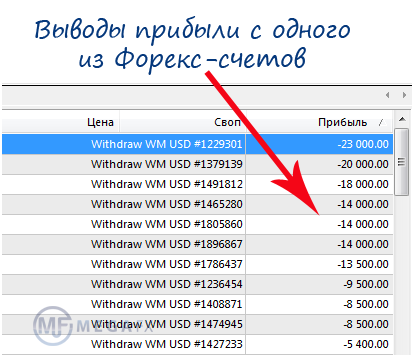
\includegraphics[width=0.75\linewidth]{img/concl}

% \TODO